%章节
%\section{}, \subsection{}, \subsubsection{}, \paragraph{}, \subparagraph{}

%插入图片
%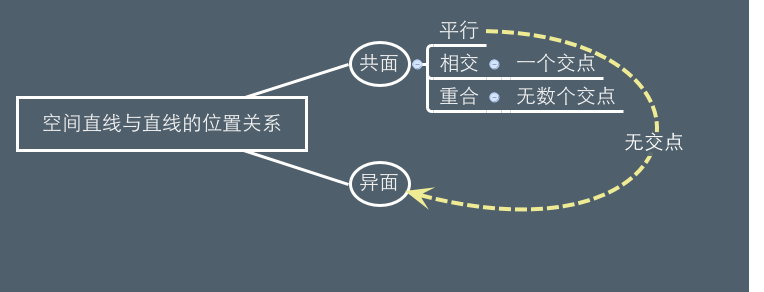
\includegraphics[height=100px]{/Users/shuyue/Desktop/1.png}

%无序列表
%\begin{itemize}
%\item
%\item
%\item
%\item 
%\end{itemize}

%有序列表
%\begin{enumerate}
%\item 
%\item
%\item
%\item
%\end{enumerate}

%嵌套列表
%\begin{itemize}
%\item
%\begin{enumerate}
%\item 
%\item 
%\item 
%\end{enumerate}
%\item
%\begin{enumerate}
%\item 
%\item 
%\item 
%\end{enumerate}
%\end{itemize}

%分栏
%\begin{multicols}{2}
%1\columnbreak \\ 2
%\end{multicols}

%标号
%\textcircled{1}

\documentclass[a4,12pt]{article}
\RequirePackage{CJKutf8,hyperref,mathtools,amssymb,geometry,enumerate,multicol,graphicx,dcolumn}

\begin{document}
\begin{CJK}{UTF8}{gkai}

\title{小数的简便运算}
\date{}
\author{张舒悦}
\maketitle

\section{教学目标}
\begin{enumerate}
\item 知道自然数加法运算定律, 减法运算性质对于小数同样适用.
\item 能运用加法运算定律, 减法运算性质使一些小数运算简便.
\end{enumerate}

\section{教学重点}
\begin{enumerate}
\item 正确进行小数加减混合运算.
\end{enumerate}

\section{教学难点}
\begin{enumerate}
\item 能运用加法运算定律, 减法运算性质使一些小数计算简便.
\end{enumerate}

\section{教学过程}

\subsection{引入}
回顾关于加减法的运算定律, 运算性质.\\
加法交换律:$$a+b=b+a.$$
加法结合律:$$a+b+c=a+(b+c).$$
减法运算性质:$$a-b-c=a-(b+c).$$
\subsection{例题1}
$$25.2-8.8-4.2$$
法一: 利用同级运算可交换.
\begin{align*}
&25.2-8.8-4.2\\
=&25.2-4.2-8.8\\
=&21-8.8\\
=&12.2
\end{align*}\\
简便之处为小数部分相同的小数相减.\\
\vspace{8mm}
\\法二: 利用减法运算性质.
\begin{align*}
&25.2-8.8-4.2\\
=&25.2-(4.2+8.8)\\
=&25.2-13\\
=&12.2
\end{align*}
简便之处为小数部分可凑整的小数相加.

\subsection{练习1}
\begin{align*}
&3.7-0.72+7.3\\
=&3.7+7.3-0.72\\
=&11-0.72\\
=&10.28
\end{align*}

\subsection{例题2}
依次利用加法交换律与加法结合律.
\begin{align*}
&37.63+46.24+43.37+40.76\\
=&(37.63+43.37)+(46.24+40.76)\\
=&81+87\\
=&168
\end{align*}\\
简便之处为小数部分可凑整的小数相加.

\subsection{练习2}
\begin{align*}
&13.51+4.72-0.51+5.28\\
=&(13.51-0.51)+(4.72+5.28)\\
=&13+10\\
=&23
\end{align*}

\subsection{书后练习}
递等式计算, 面批.

\subsection{思考题}
\begin{align*}
&0.723 \times 0.62+0.62 \times 0.277 \\
=&0.62 \times (0.723+0.277)\\
=&0.62 \times 1\\
=&0.62
\end{align*}

\section{小结}
\begin{enumerate}
\item 简便之处{\begin{itemize}
\item 小数部分相同的小数相减.
\item 小数部分可凑整的小数相加.
\end{itemize}}
\item 加减运算定律或性质{\begin{itemize}
\item 加法交换律.
\item 加法结合律.
\item 减法运算性质.
\item 同级运算可交换顺序.
\end{itemize}}
\end{enumerate}

\section{作业}
\begin{enumerate}
\item 订正练习册和一课一练
\item 一课一练P57-58
\item 练习册P32
\end{enumerate}


\end{CJK}
\end{document}